\documentclass[12pt,letterpaper]{article}
\usepackage[utf8]{inputenc}
\usepackage{amsmath}
\usepackage{amsfonts}
\usepackage{amssymb}
\usepackage{amsthm}
\usepackage{graphicx}

\usepackage{hyperref}
\hypersetup{
    colorlinks=true,
    linkcolor=blue,
    filecolor=magenta,      
    urlcolor=cyan,
}
\urlstyle{same}

\usepackage{tabularx}
\usepackage[left=2cm,right=2cm,top=2cm,bottom=2cm]{geometry}
\usepackage{fancyhdr}
\usepackage{multicol}
\usepackage{multirow,array}
\usepackage{newtxtext,newtxmath}
\usepackage{relsize}
\usepackage{lastpage}
\usepackage{enumitem}
\usepackage{adjustbox}
\newcolumntype{Y}{>{\centering\arraybackslash}X}
\pagestyle{fancy}
\fancyhf{}
\lhead{\textsc{BHCC Mat-181}}
\chead{\textsc{Answers}}
\rhead{\textsc{Exercises 2.15-2.21}}
\rfoot{Page \thepage ~of \pageref*{LastPage}}
\setenumerate[1]{label={\bf 2.\theenumi: }}
\setenumerate[2]{label={\bf (\theenumii): }}
\setenumerate[3]{label={\bf \theenumiii: }}

\begin{document}
\newcommand{\AND}{~\textsc{and}~}
\newcommand{\OR}{~\textsc{or}~}

\begin{enumerate}
\setcounter{enumi}{14}
\item \begin{enumerate}
\item No.
\item \begin{enumerate}
	\item If $A$ and $B$ are independent, then 
	\begin{align*}
	P(A\AND B) &= P(A) \cdot P(B) \\
	&= 0.3 \cdot 0.7 \\
	&= \fbox{0.21} \\
	\end{align*}
	\item By continuing to assume independence, we can use 0.21 in the general Addition Rule.
	\begin{align*}
	P(A\OR B) &= P(A) + P(B) - P(A\AND B) \\
	&= 0.3 + 0.7 - 0.21 \\
	&= \fbox{0.79} \\
	\end{align*}
	\item When $A$ and $B$ are independent, then $P(A|B) = P(A)$. 
	$$P(A|B) = \fbox{0.3} $$
\end{enumerate}
\item No. If ~$P(A\AND B) \ne P(A) \cdot P(B)$ ~ then $A$ and $B$ are independent.
$$0.1 \ne 0.3 \cdot 0.7$$
\item We can use the definition of conditional probability.
\begin{align*}
P(A | B) &= \frac{P(A\AND B)}{P(B)} \\\\
&= \frac{0.1}{0.3} \\\\
&\approx \fbox{0.33} \\
\end{align*}
\end{enumerate}

\item We can use the definition of conditional probability.
\begin{align*}
P(\text{jelly}|\text{pb}) &= \frac{P(\text{jelly}\AND\text{pb})}{P(\text{pb})} \\\\
&= \frac{0.78}{0.8}\\\\
&= \fbox{0.975}
\end{align*}

\newpage
\item \begin{enumerate}
	\item No. The joint probability is 0.18. Disjoint (mutually exclusive) events have a zero joint probability.
	\item We refer to the Addition Rule:
	\begin{align*}
	P(A\OR B) &= P(A) + P(B) - P(A\AND B) \\
	&= 0.6 + 0.2 - 0.18 \\
	&= \fbox{0.78} \\
	\end{align*}
	\item We refer to the definition of conditional probability:
	\begin{align*}
	P(A | B) &= \frac{P(A\AND B)}{P(B)}  \\\\
	&= \frac{0.18}{0.2} \\\\
	&= \fbox{0.9} \\
	\end{align*}
	\item We refer to the definition of conditional probability:
	\begin{align*}
	P(A | B) &= \frac{P(A\AND B)}{P(B)}  \\\\
	&= \frac{0.11}{0.33} \\\\
	&\approx \fbox{0.33} \\
	\end{align*}
	\item It appears that liberal democrats are more likely to believe in global warming, so belief in warming and party are {\bf not} independent.
	\item We refer to the definition of conditional probability:
	\begin{align*}
	P(A | B) &= \frac{P(A\AND B)}{P(B)}  \\\\
	&= \frac{0.06}{0.34} \\\\
	&\approx \fbox{0.18} \\
	\end{align*}
\end{enumerate}

\newpage
\item \begin{enumerate}
	\item No. Their joint probability is not 0.
	\item 0.2329
	\item $\frac{0.2099}{0.8738} \approx \fbox{0.24} $
	\item $\frac{0.0230}{0.1262} \approx \fbox{0.18} $
	\item Nope, otherwise answers to (c) and (d) would be the same.
\end{enumerate}

\item \begin{enumerate}
	\item No. Their joint probability is not 0.
	\item $\frac{162}{248} \approx \fbox{0.65}$
	\item $\frac{181}{252} \approx \fbox{0.72} $
	\item To answer this, we need to assume that their tastes are independent and that they are represented by this poll. $$P(\text{``man likes In-N-Out}\AND\text{``woman likes In-N-Out}) = 0.65 \cdot 0.72 \approx 0.47  $$
	\item $\frac{252+6-1}{500} = 0.514$
\end{enumerate}

\item \begin{enumerate}
	\item $\frac{108+114-78}{204} \approx \fbox{0.706} $
	\item $\frac{78}{114} \approx \fbox{0.684} $
	\item $\frac{19}{54} \approx \fbox{0.352} $ \\
	      $\frac{11}{36} \approx \fbox{0.306} $
	\item They do not seem independent. Whether the woman has blue eyes depends on whether the man has blue eyes.
\end{enumerate}

\item \begin{enumerate}
	\item Tree diagram:
	\begin{center}
	\includegraphics[scale=0.6]{figures/tree.png}
	\end{center}
	\item $\frac{0.688}{0.688+0.13} = \fbox{0.84}$
\end{enumerate}

\end{enumerate}
\end{document}